% 2013 全国卷Ⅰ文科第 22 题：圆、切线、角平分线及弦。
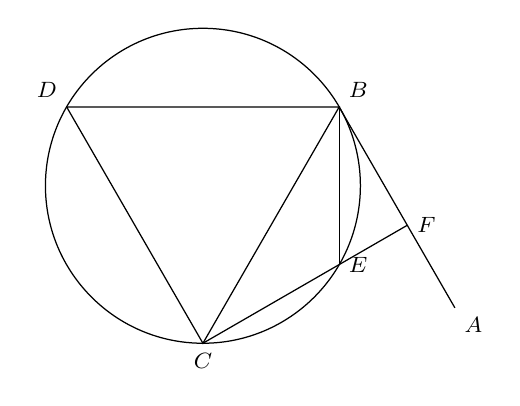
\begin{tikzpicture}[font=\footnotesize, line width=0.45pt]
  \coordinate (O) at (0,0);
  \coordinate (B) at (1.73,1.00);
  \coordinate (D) at (-1.73,1.00);
  \coordinate (C) at (0,-2.00);
  \coordinate (E) at (1.73,-1.00);
  \coordinate (F) at (2.598,-0.50);
  \coordinate (A) at (3.20,-1.55);
  \draw (O) circle (2);
  \draw (D)--(B)--(C)--(D);
  \draw (B)--(E);
  \draw (C)--(F);
  \draw (B)--(A);
  \node[above right] at (B) {$B$};
  \node[above left] at (D) {$D$};
  \node[below] at (C) {$C$};
  \node[right] at (E) {$E$};
  \node[right] at (F) {$F$};
  \node[below right] at (A) {$A$};
\end{tikzpicture}
